\documentclass{article}
\usepackage[T1]{fontenc}
\usepackage{lmodern}
\usepackage{graphicx}
\usepackage{amsmath,amssymb}
\usepackage[a4paper,margin=2cm]{geometry}
\usepackage[absolute,overlay]{textpos}
\setlength{\TPHorizModule}{1mm}
\setlength{\TPVertModule}{1mm}
\usepackage[indonesian]{babel}
\usepackage{hyperref}
\setlength{\emergencystretch}{2em}
% unit: Halaman 2

\begin{document}

% === Halaman 2 (llm) ===

\section*{Steganalysis}

\vspace{101.57mm}

\begin{itemize}
    \item Tujuan: menentukan apakah sebuah media \textit{suspect} mengandung pesan tersembunyi
\end{itemize}

\vspace{10mm}

% deskripsi: Ilustrasi proses steganalysis yang menunjukkan penggunaan kaca pembesar untuk melihat nilai-nilai piksel (angka digital) di dalam sebuah gambar wajah seseorang.
% bbox normalisasi: [0.2910, 0.4560, 0.5930, 0.7980]
\begin{textblock*}{63.42mm}(61.11mm,135.43mm)
\noindent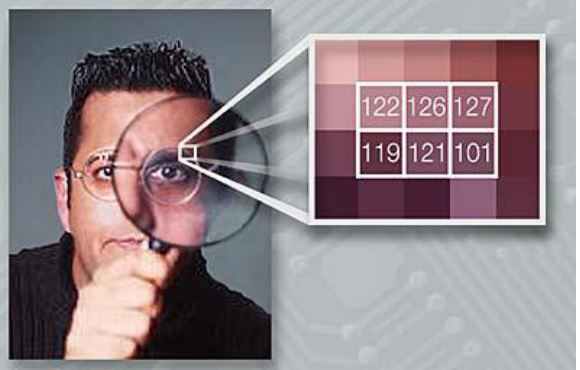
\includegraphics[width=63.42mm,height=101.57mm]{../../images/llm/page_002_img_01.png}%
\end{textblock*}

\end{document}
